\chapter{Практические задания}

\section{Асинхронный RS-триггер}

Асинхронный RS-триггер является простейшим триггером, служащим запоминающей ячейкой. Ниже, на рисунке \ref{async-rs}, представлена схема такого триггера.

\begin{figure}
	\centering
	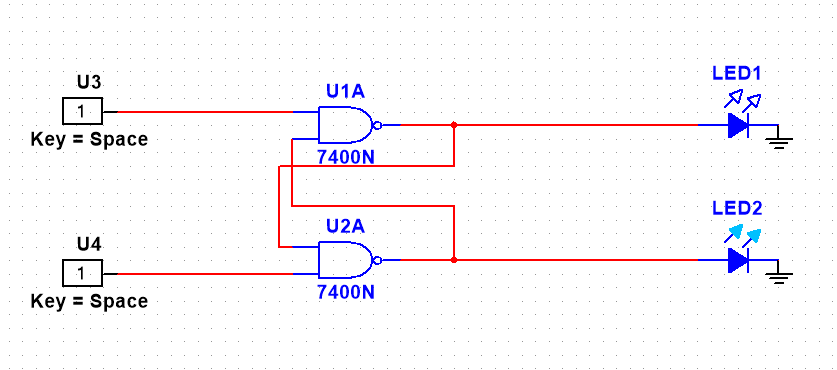
\includegraphics[width=\linewidth]{rs-nand.png}
	\caption{Схема асинхронного RS-триггера}
	\label{async-rs}
\end{figure}

Изменяя необходимые сигналы на входах $\overline{S}$ и $\overline{R}$ триггера, составим таблицу переходов (таблица \ref{async-rs-table}).

\begin{table}
	\centering
	\caption{Таблица переходов асинхронного RS-триггера}
	\begin{tabular}{|c|c|c|c|c|}
		\hline
		$~~~~~\overline{S}~~~~~$ & $~~~~~\overline{R}~~~~~$ & $~~~~~Q_{t-1}~~~~~$ & $~~~~~Q_t~~~~~$ & Значение \\
		\hline
		$0$ & $0$ & $0$ & $X$ &  \multirow{2}{*}{Запрещенное состояние} \\
		\cline{1-4}
		$0$ & $0$ & $1$ & $X$ & \\
		\hline
		$0$ & $1$ & $0$ & $1$ &  \multirow{2}{*}{Установка 1} \\
		\cline{1-4}
		$0$ & $1$ & $1$ & $1$ & \\
		\hline
		$1$ & $0$ & $0$ & $0$ &  \multirow{2}{*}{Установка 0} \\
		\cline{1-4}
		$1$ & $0$ & $1$ & $0$ & \\
		\hline
		$1$ & $1$ & $0$ & $0$ &  \multirow{2}{*}{Хранение} \\
		\cline{1-4}
		$1$ & $1$ & $1$ & $1$ & \\
		\hline
	\end{tabular}
	\label{async-rs-table}
\end{table}

\pagebreak

\section{Синхронный RS-триггер}

В отличие от асинхронного триггера, синхронный имеет вход синхронизации $C$, в дополнении к двум входам управления ($R$ и $S$). При $C = 1$ синхронный RS-триггер работает как асинхронный.

Схема синхронного RS-триггера представлена на рисунке \ref{sync-rs}

\begin{figure}
	\centering
	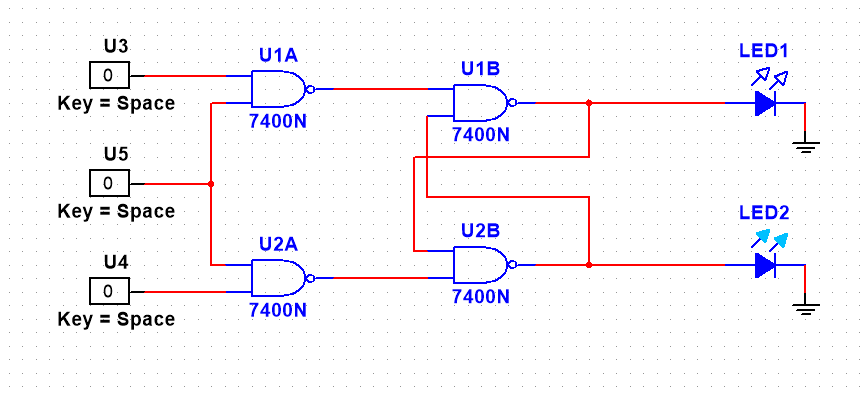
\includegraphics[width=\linewidth]{sync_nand.png}
	\caption{Схема синхронного RS-триггера}
	\label{sync-rs}
\end{figure}

Ниже (таблица \ref{sync-rs-table}) представлена таблица переходов синхронного RS-триггера.

\begin{table}
	\centering
	\caption{Таблица переходов синхронного RS-триггера}
	\begin{tabular}{|c|c|c|c|c|c|}
		\hline
		$~~~~~C~~~~~$ & $~~~~~S~~~~~$ & $~~~~~R~~~~~$ & $~~~~~Q_{t-1}~~~~~$ & $~~~~~Q_t~~~~~$ & Значение \\
		\hline
		$0$ & $\forall$ & $\forall$ & $Q_{t-1}$ & $Q_{t-1}$ & \multirow{3}{*}{Хранение} \\
		\cline{1-5}
		$1$ & $0$ & $0$ & $0$ & $0$ & \\
		\cline{1-5}
		$1$ & $0$ & $0$ & $1$ & $1$ & \\
		\hline
		$1$ & $0$ & $1$ & $0$ & $0$ &  \multirow{2}{*}{Установка 0} \\
		\cline{1-5}
		$1$ & $0$ & $1$ & $1$ & $0$ & \\
		\hline
		$1$ & $1$ & $0$ & $0$ & $1$ &  \multirow{2}{*}{Установка 1} \\
		\cline{1-5}
		$1$ & $1$ & $0$ & $1$ & $1$ & \\
		\hline
		$1$ & $1$ & $1$ & $0$ & $X$ &  \multirow{2}{*}{Запрещенное состояние} \\
		\cline{1-5}
		$1$ & $1$ & $1$ & $1$ & $X$ & \\
		\hline
	\end{tabular}
	\label{sync-rs-table}
\end{table}

\pagebreak

\section{Синхронный D-триггер}

Синхронный D-триггер имеет один информационный вход D, состояние которого с каждым синхронизирующим импульсом передается на выход. Сигналы -- задержанные входные сигналы.

Ниже, на рисунке \ref{d-sync}, представлена схема синхронного D-триггера.

\begin{figure}
	\centering
	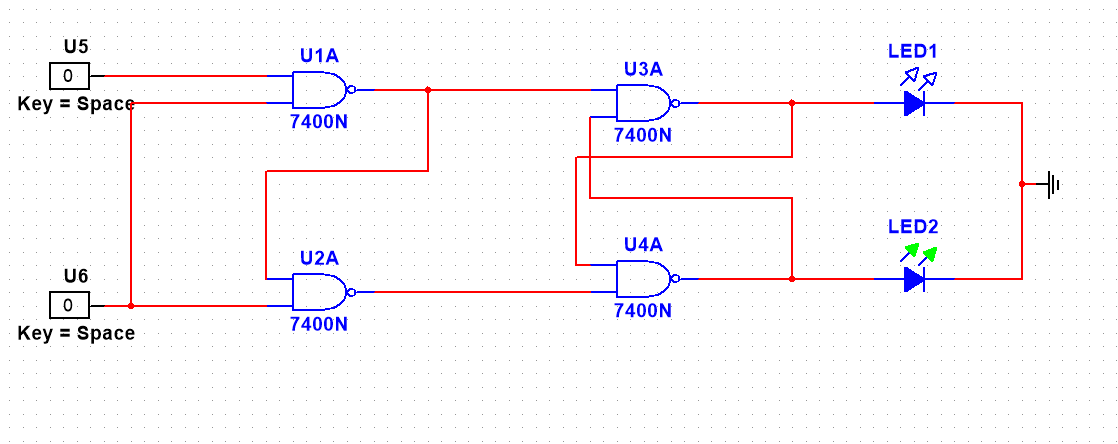
\includegraphics[width=\linewidth]{d-sync.png}
	\caption{Схема синхронного D-триггера}
	\label{d-sync}
\end{figure}

Таблица \ref{d-sync-table} переходов для синхронного D-триггера представлена ниже.

\begin{table}
	\centering
	\caption{Таблица переходов синхронного D-триггера}
	\begin{tabular}{|c|c|c|c|c|}
		\hline
		$~~~~~C~~~~~$ & $~~~~~D~~~~~$ & $~~~~~Q_{t-1}~~~~~$ & $~~~~~Q_t~~~~~$ & Значение \\
		\hline
		$0$ & $0$ & $0$ & $0$ &  \multirow{4}{*}{Хранение} \\
		\cline{1-4}
		$0$ & $0$ & $1$ & $1$ & \\
		\cline{1-4}
		$0$ & $1$ & $0$ & $0$ & \\
		\cline{1-4}
		$0$ & $1$ & $1$ & $1$ & \\
		\hline
		$1$ & $0$ & $0$ & $0$ &  \multirow{2}{*}{Установка 0} \\
		\cline{1-4}
		$1$ & $0$ & $1$ & $0$ & \\
		\hline
		$1$ & $1$ & $0$ & $1$ &  \multirow{2}{*}{Установка 1} \\
		\cline{1-4}
		$1$ & $1$ & $1$ & $1$ & \\
		\hline
	\end{tabular}
	\label{d-sync-table}
\end{table}

\pagebreak

\section{Синхронный D-триггер с динамическим управлением записью}

В отличие от обычного синхронного D-триггера, состояние D-триггера с динамическим управлением записью меняется по фронту синхросигнала. Схему данного триггера можно увидеть на рисунке \ref{d-dyn}.

\begin{figure}
	\centering
	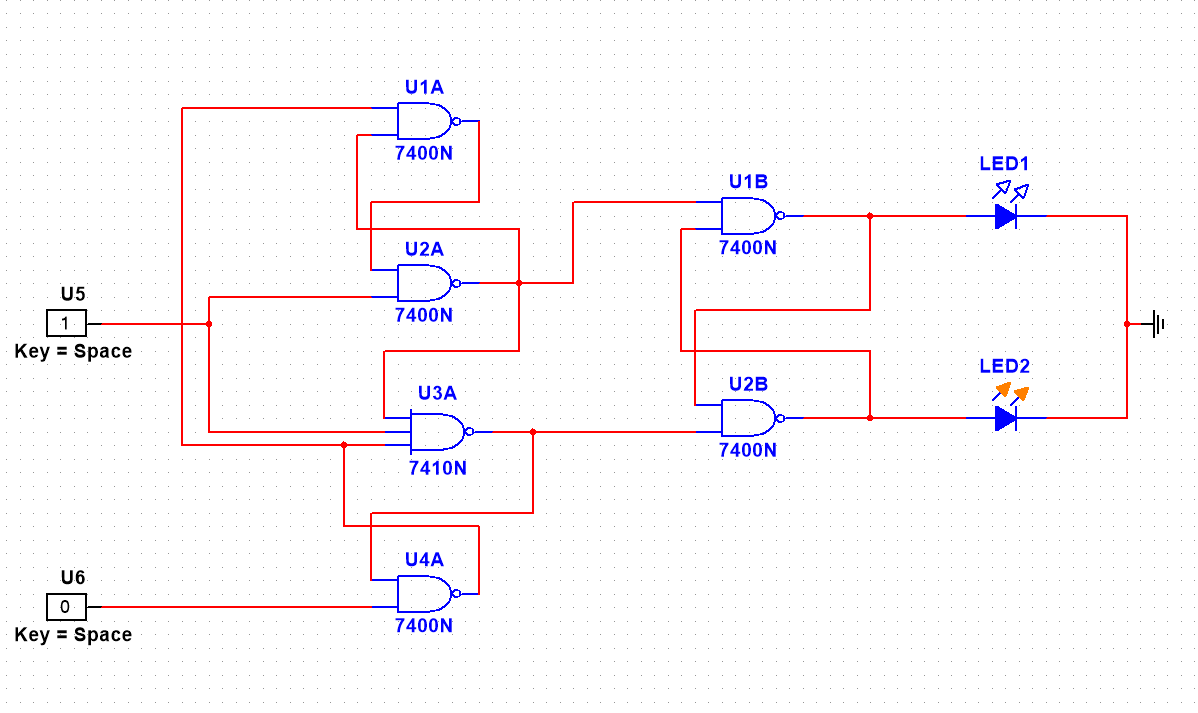
\includegraphics[width=\linewidth]{d_dyn.png}
	\caption{Схема синхронного D-триггера с динамическим управлением}
	\label{d-dyn}
\end{figure}

Таблица \ref{d-dyn-table} переходов для синхронного D-триггера представлена ниже.

\begin{table}
	\centering
	\caption{Таблица переходов синхронного D-триггера с динамическим управлением}
	\begin{tabular}{|c|c|c|}
		\hline
		$~~~~~D~~~~~$ & $~~~~~C~~~~~$ & $~~~~~Q~~~~~$ \\
		\hline
		$0$ & $0 \rightarrow 1$ & $0$ \\
		\hline
		$1$ & $0 \rightarrow 1$ & $1$ \\
		\hline
		$0$ & $0$ & $0$ \\
		\hline
		$1$ & $0$ & $1$ \\
		\hline
		$0$ & $1$ & $0$ \\
		\hline
		$1$ & $1$ & $1$ \\
		\hline
	\end{tabular}
	\label{d-dyn-table}
\end{table}

\pagebreak

\section{Синхронный DV-триггер с динамическим управлением записью}

При $C = 0$ DV-триггер, как и синхронные триггеры всех типов, сохраняет предыдущее внутреннее состояние ($Q_{n+1} = Q_n$). При $C = 1$ и при наличии сигнала $V = 1$ разрешения приема информации, DV-триггер принимает информационный сигнал, действующий на входе D, т. е. работает как асинхронный DV-триггер. При $C = 1$ и $V = 0$ DV-триггер сохраняет предыдущее внутреннее состояние.

Схема DV-триггера с динамическим управлением записью представлена на рисунке \ref{dv}.

\begin{figure}
	\centering
	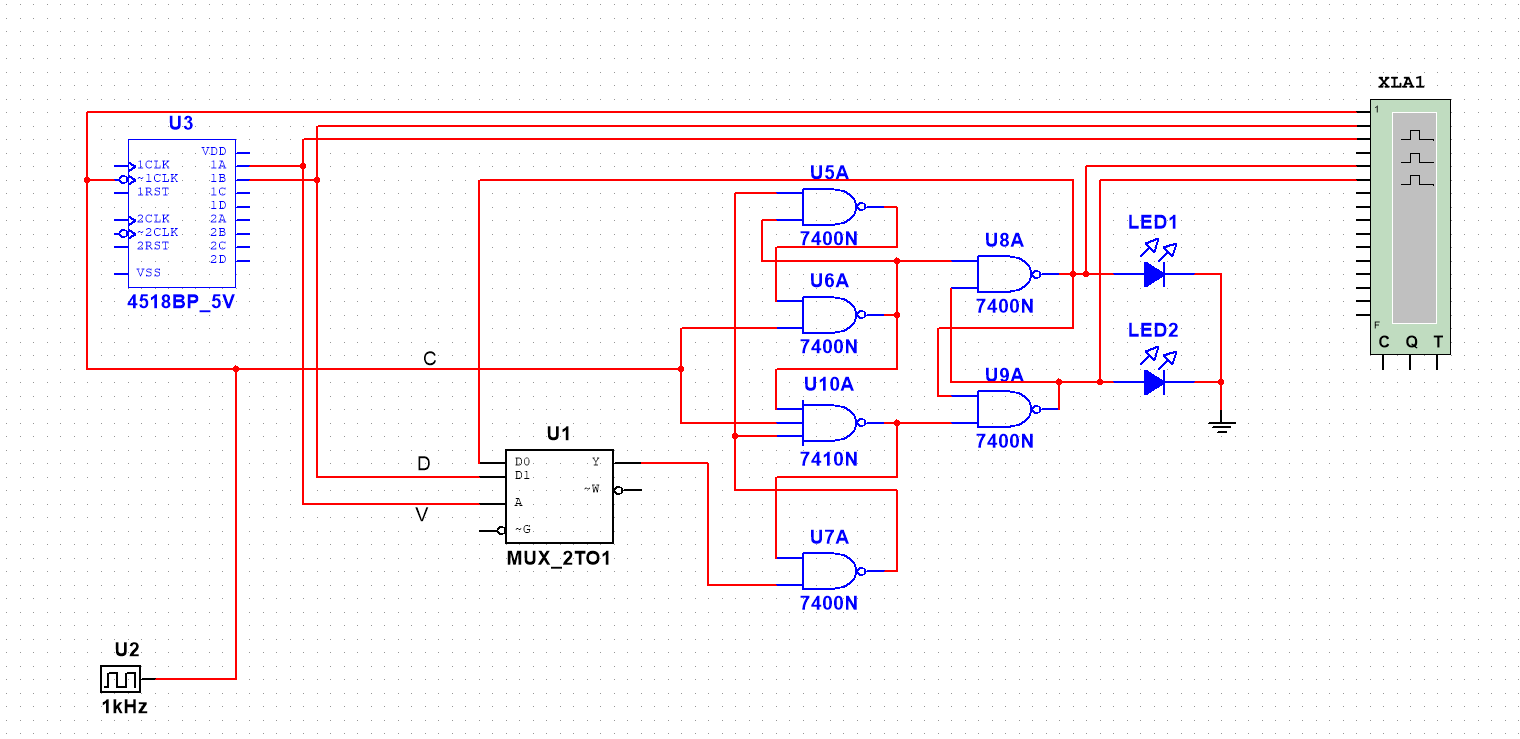
\includegraphics[width=\linewidth]{DV.png}
	\caption{Схема синхронного DV-триггера с динамическим управлением}
	\label{dv}
\end{figure}

Ниже, на рисунке \ref{dv-diag}, представленны временные диаграммы синхронного DV-триггера.

\begin{figure}
	\centering
	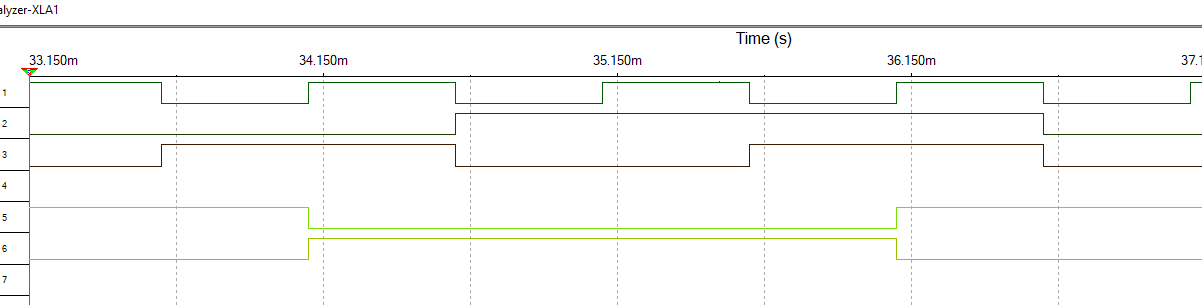
\includegraphics[width=\linewidth]{DV_anal.png}
	\caption{Временные диаграммы синхронного DV-триггера с динамическим управлением}
	\label{dv-diag}
\end{figure}

\pagebreak

\section{DV-триггер, включенный по схеме TV-триггера}

TV-триггер кроме счётного входа Т имеет второй, управляющий, V-вход для разрешения приёма информации. TV-триггер называют тактируемым или синхронным счётным триггером. Состояние TV-триггера меняется по фронту разрешающего сигнала V. Ниже, на рисунке \ref{tv}, представлена схема получения TV-триггера из DV-триггера с динамическим управлением записью.

\begin{figure}
	\centering
	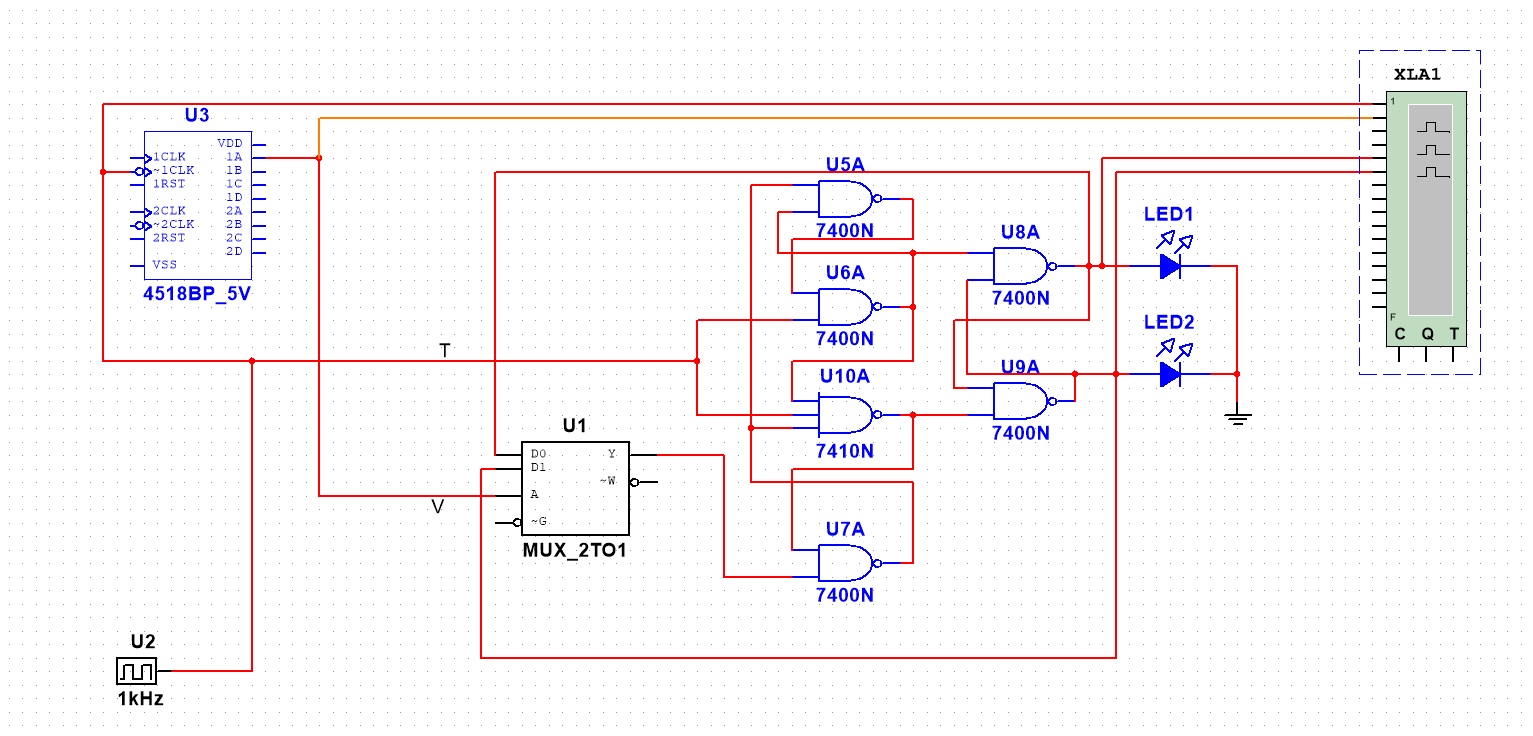
\includegraphics[width=\linewidth]{TV.png}
	\caption{Схема TV-триггера}
	\label{tv}
\end{figure}

Ниже, на рисунке \ref{tv-diag}, представленны временные диаграммы TV-триггера.

\begin{figure}
	\centering
	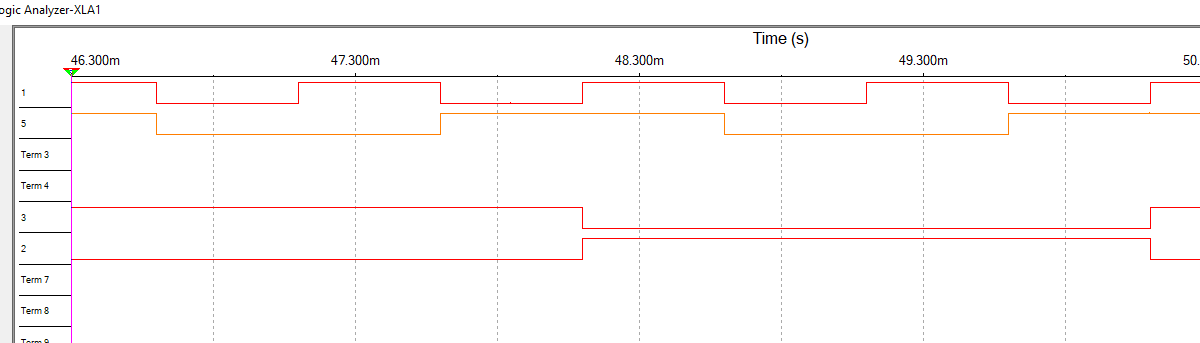
\includegraphics[width=\linewidth]{TV_anal.png}
	\caption{Временные диаграммы TV-триггера}
	\label{tv-diag}
\end{figure}

\pagebreak

\chapter{Контрольные вопросы}

\begin{enumerate}
	\item Что называется триггером? \\
	Триггер является запоминающим элементом с двумя устойчивыми состояниями, которые
	кодируются цифрами 0 и 1.
	\item Какова структурная схема триггера? \\
	Структурная схема триггера представлена ниже, на рисунке \ref{struct}
	\begin{figure}
		\centering
		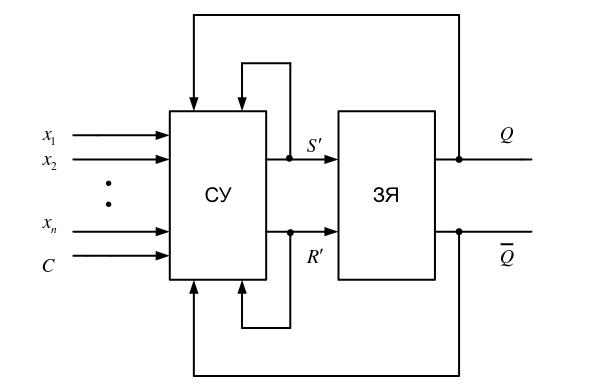
\includegraphics[width=0.7\linewidth]{struct.png}
		\caption{Структурная схема триггера}
		\label{struct}
	\end{figure} 
	\item По каким основным признакам классифицируют триггеры? \\ 
	Триггеры классифицируют:\\ По способу организации логических связей, т.е. по виду логического уравнения,
	характеризующего состояние входов и выходов триггера в момент времени $t_n$ до его
	срабатывания и в момент $t_{n+1}$ после его срабатывания, различают триггеры:
	\begin{itemize}
		\item  с раздельной установкой состояний “0” и “1” (RS-триггеры);
		\item  со счетным входом (Т-триггеры);
		\item  универсальные с раздельной установкой состояний “0” и “1” (JK-триггеры);
		\item  с приемом информации по одному входу (D триггеры);
		\item  универсальные с управляемым приемом информации по одному входу (DV-триггеры);
		\item  комбинированные (например, RST-, JKRS, DRS-триггеры) и т.д.\\
		По способу запаси информации различают триггеры:
		\item  асинхронные (не синхронизируемые);
		\item  синхронные (синхронизируемые), или тактируемые.
	\end{itemize}
	По способу синхронизации различают триггеры: синхронные со статическим управлением
	записью; синхронные с динамическим управлением записью.\\
	По способу передачи информации с входов на выход различают триггеры о
	одноступенчатым и двухступенчатым запоминанием информации.
	\item Каково функциональное назначение входов триггеров? \\
	S-вход − вход для раздельной установки триггера в состояние "1" (Set – установка)\\
R-вход − вход для раздельной установки триггера в состояние "0" (Reset – сброс, очистка)\\
J-вход − вход для установки состояния "1" в универсальном JK-триггере (Jerk – внезапное
включение)\\
K-вход − вход для установки состояния "0" в универсальном JK-триггере (Kill – внезапное
отключение)\\
D-вход −информационный вход для установки триггера в состояния "1" или "0" (Data – данные,
Delay – задержка)\\
V-вход − подготовительный управляющий вход для разрешения приема информации (Valve –
клапан, вентиль)\\
C-вход - исполнительный управляющий (командный) вход для осуществления приема
информации, вход синхронизации (Clock – источник синхросигналов)
	\item Что такое асинхронный и синхронный триггеры? \\
	Асинхронный RS -триггер - это простейший триггер, который
используется как запоминающая ячейка.\\
Синхронный RS-триггер имеет два информационных входа R и S и вход
синхронизации С.
	\item Что такое таблица переходов? \\
	Таблица переходов отражает зависимость выходного сигнала триггера в
момент времени $t_{n+1}$ от входных сигналов и от состояния триггера в
предыдущий момент времени tn.
	\item Как работает асинхронный RS-триггер? \\
	при $S = 0$ и $R = 1$ триггер устанавливается в состояние "0", а при $S = 1$ и $R =
0$ - в состояние “1”, если $S = 0$ и $R = 0$, то в триггере сохраняется
предыдущее внутреннее состояние.
	\item Как работает синхронный RS -триггер? Какова его таблица переходов? \\
	Как и все синхронные триггеры, синхронный RS - триггер при $C = 0$
сохраняет предыдущее внутреннее состояние, т.е. $Q_{n+1}$ = $Q_n$ . Сигналы по
входам S и R переключают синхронный RS-триггер только с
поступлением импульса на вход синхронизации С. При $C = 1$ синхронный
триггер переключается как асинхронный. Одновременная подача
сигналов $C = S = R= 1$ запрещена. При $S = R = 0$ триггер не изменяет своего
состояния.

Таблица переходов представлена выше (таблица \ref{sync-rs-table}).
	\item Что такое D-триггер? \\
	Синхронный D-триггер имеет один информационный вход D, состояние
которого с каждым синхронизирующим импульсом передается на выход,
т.е. выходные сигналы представляют собой задержанные входные
сигналы. Поэтому D-триггер – элемент задержки (хранения) входных
сигналов на один такт.
	\item Объясните работу синхронного D-триггера. \\
	сигнал D на вход S, а сигнал , т.е. с выхода инвертора сигнала D, на вход
R. В результате на входах RS-триггера возможны только наборы сигналов
$SR = 01$ при $D=0$ или $SR =10$ при $D=1$, что соответствует записи в триггер
логического 0 или 1. Путем логических преобразований инвертор можно
исключить и получить схему синхронного D–триггера. Синхронный
D-триггер имеет один информационный вход D, состояние которого с
каждым синхронизирующим импульсом передается на выход, т. е.
выходные сигналы представляют собой задержанные входные сигналы.
	\item Что такое DV–триггер? \\
	Синхронный DV-триггер имеет один информационный
вход D и один подготовительный разрешающий вход V для разрешения
приема информации.
	\item Объясните работу DV-триггера. \\
	При $C = 0$ DV-триггер, как и синхронные триггеры всех типов, сохраняет
предыдущее внутреннее состояние, т.е. $Q_{n+1} = Q_n$ . При $C = 1$ и при наличии
сигнала $V = 1$ разрешения приема информации DV-триггер принимает
информационный сигнал, действующий на входе D, т.е. работает как
асинхронный DV-триггер. При $C = 1$ и $V = 0$ DV-триггер сохраняет
предыдущее внутреннее состояние, т.е. $Q_{n+1} = Q_n$ .
	\item Что такое T-триггер? Какова его таблица переходов? \\
	Т-триггер имеет один информационный вход Т, называемый счетным
входом. Асинхронный Т-триггер переходит в противоположное состояние
каждый раз при подаче на Т-вход единичного сигнала. Таким образом
Т-триггер реализует счет по модулю 2: $Q_t = T_{t-1} \oplus Q_{t-1}$. Синхронный Т-триггер имеет
вход С и вход Т. Синхронный Т-триггер переключается в
противоположное состояние сигналом С, если на счетном входе Т
действует сигнал логической 1.


	\item Объясните работу схемы синхронного RS-триггера со статическим управлением. \\
	При $C = 0$ триггеры переходят в режим хранения, запоминая последнее состояние
	\item Какова характерная особенность переключения синхронных триггеров с динамическим управлением записью? \\
	Характерной особенностью синхронных триггеров с динамическим управлением записью
является то, что прием информационных сигналов и передача на выход принятой информации
выполняются в момент изменения синхросигнала на С-входе из 0 в 1 или из 1 в 0, т.е.
перепадом синхросигнала
	\item Как работает схема синхронного D -триггера с динамическим управлением записью на основе трех RS-триггеров? \\
	Триггер имеет асинхронные входы $S_a$ и $R_a$ начальной установки в состояния 1 и 0. Если схему
D-триггера дополнить входом V, то получим структуру DV-триггера. Временные диаграммы D-триггера соответствуют временным диаграммам DV-триггера при $V = 1$.
	\item Составьте временные диаграммы работы синхронного D-триггера с динамическим управлением записью.
	\item Какова структура и принцип действия синхронного DV-триггера с динамическим управлением записью? \\
	Синхронный DV-триггер имеет один информационный вход D и один подготовительный
разрешающий вход V для разрешения приема информации.
	\begin{equation}
		Q_t = DV + \underline{V}Q_{t-1} = DVC + (\underline{V} + \underline{C})Q_{t-1}
	\end{equation}
	При $C = 0$ DV-триггер, как и синхронные триггеры всех типов, сохраняет предыдущее внутреннее
состояние, т.е. $Q_t = Q_{t-1}$. При $C = 1$ и при наличии сигнала $V = 1$ разрешения приема информации
DV-триггер принимает информационный сигнал, действующий на входе D, т.е. работает как
асинхронный DV-триггер. При $C = 1$ и $V = 0$ DV-триггер сохраняет предыдущее внутреннее
состояние.
	\item Составьте временные диаграммы синхронного DV-триггера.
	\item Объясните режимы работы D-триггера. \\
	Синхронный D-триггер имеет один информационный вход D, состояние которого с каждым
синхронизирующим импульсом передается на выход, т. е. выходные сигналы представляют
собой задержанные входные сигналы.

\end{enumerate}
